% Paper 4 --- legislative churn in Saudi legislation.
% Footnote citations, double-spacing applied at build time, venue-neutral
% until one is chosen. Compiles on a plain TeX Live; build.py produces the
% submission files.
\documentclass[11pt]{article}
\usepackage[a4paper,top=2.5cm,bottom=2.5cm,left=3cm,right=3cm]{geometry}
\usepackage{times}
\usepackage{setspace}
\onehalfspacing
\usepackage[hidelinks]{hyperref}

% Set \anontrue before producing the file uploaded to a journal that reviews
% anonymously.

\usepackage[T1]{fontenc}
\usepackage[utf8]{inputenc}
\usepackage{microtype}
\usepackage{booktabs}
\usepackage{graphicx}
\usepackage{url}
\emergencystretch=3em

\title{What Changes, and Where?\\
Legislative Churn Across Saudi Arabian Legislation}


  \author{}
  \date{}


\begin{document}

\begin{center}
{\Large\bfseries What Changes, and Where?\\[2pt]
Legislative Churn Across Saudi Arabian Legislation\par}
\end{center}
\vspace{1em}


\begin{abstract}
\noindent
Fifty-eight consecutive articles of the Saudi Law of Sharia Procedure were
repealed by a single royal decree in December 2021, and seventy-five of its
243 articles --- nearly a third --- are now repealed in total. The instrument
is still in force, still cited, and unchanged in size and numbering. How
common is that? Legal systems are usually studied as they stand at a moment,
because the evidence to study them as they move has not existed. Using a
machine-readable corpus in which 13,089 articles across 272 Saudi legislative
instruments carry a verified legal status, this article measures what
changes. Some 973 articles --- 7.4 per cent --- are no longer in their
original form: 730 amended, 138 repealed, 105 added. That change is very
unevenly spread. Nearly three-fifths of instruments record no change at all,
and the Gini coefficient of changed articles across instruments is 0.82.
Instruments change in characteristically different ways, so that a single
count of `amendments' conceals more than it reveals: one instrument is
hollowed out by repeal, another accretes new articles, a third is rewritten
in place. Two findings connect this to how a legal system is used. Instruments
that other instruments cite change substantially more than instruments nobody
cites --- 10.7 per cent against 6.1 per cent, rising to 13.4 per cent for the
fifteen most cited --- although age is not controlled for and may explain some
of it. And cross-instrument references are more than twice as likely as the
base rate to point at an article that has since changed, while an instrument's
references to its own articles are not: drafters maintain their own internal
references and cannot maintain anyone else's.
\end{abstract}

\vspace{1em}\noindent\textbf{Keywords:} legislative amendment; consolidation;
statutory maintenance; Saudi Arabia; legal corpora; empirical legal studies
\vspace{1.5em}

\section{Introduction}

On 26/5/1443H --- 30 December 2021 --- a single royal decree issued the Saudi
Evidence Law, 129 articles in eleven chapters.\footnote{Evidence Law (Royal
Decree M/43, 26/5/1443H).} The same decree repealed articles 101 to 158 of the
Law of Sharia Procedure: fifty-eight consecutive articles, the whole of that
instrument's treatment of proof, lifted out and re-enacted elsewhere. Two
later decrees repealed ten more. Seventy-five of the Law of Sharia Procedure's
243 articles are now repealed --- nearly a third of the instrument --- and
none of this is visible in its shape. It remains in force, its articles are
still numbered 1 to 243, and a reader who does not check the status of each
article will not discover which of them still say anything.

This is not a defect peculiar to one statute. It is what a working legal
system looks like from the inside. Statutes are amended, articles are
repealed, new articles are inserted, and the instrument a reader holds is a
composite of enactments made across decades. Every legal system does this.
What no legal system has been able to say, until recently and for very few
jurisdictions, is how much of it does it, where, and how far.

The obstacle is evidential. Measuring change requires knowing, for each
article, whether it is the article originally enacted --- and legal databases
usually present the consolidated current text, silently. The history is
either absent, or present as prose a human must read. We are aware of no Arab
jurisdiction for which the question has been asked at corpus scale, and of few
studies anywhere that ask it at the level of the individual article.

This article asks it for Saudi Arabia. It uses a corpus in which every article
verified against an official source carries a legal status --- original,
amended, repealed or added --- covering 13,089 articles across 272
instruments.\footnote{The corpus and the scripts that reproduce every number
and figure here are openly archived; see the data availability statement.}
Saudi Arabia is a good case for the same reason it was a good case for
studying the definitional lexicon: its legislation was substantially rewritten
during the 2020s, so instruments enacted decades apart are being maintained
side by side.

Four findings follow.

First, the aggregate is small and the distribution is not. Some 973 articles,
7.4 per cent of the corpus, are no longer in their original form. But 58.8 per
cent of instruments record no change at all, and the Gini coefficient of
changed articles across instruments is 0.82. Saudi legislation does not age
evenly; a small number of instruments absorb almost all of the movement.

Second, instruments change in characteristically different ways. The Sharia
Procedure Law is dominated by repeal, the Implementing Regulation of the
Commercial Agencies Law almost entirely by addition, the VAT Regulation by
amendment in place. A single figure for `amendments' would put these three
in the same bucket, and they are not the same phenomenon: one is a
jurisdiction being transferred out, one is a regime being extended, one is a
regime being tuned.

Third, change concentrates where the system leans hardest. Instruments that
other instruments cite have a mean churn rate of 10.7 per cent against 6.1
per cent for instruments nobody cites, rising to 13.4 per cent for the fifteen
most cited. Section~\ref{sec:reliance} sets out why this is suggestive rather
than established: age is not controlled for, and it cannot be, because the
corpus dates only two of its instruments.

Fourth --- and this is the finding with the clearest practical edge ---
cross-instrument references are disproportionately exposed to change.
Seventeen per cent of the references from one instrument to a specific article
of another point at an article that has since been amended or repealed,
against a corpus base rate of 7.4 per cent. References an instrument makes to
its own articles show no such excess. The asymmetry has an obvious mechanism:
a drafter amending an instrument can see and fix the references inside it,
and has no way to find the references to it.

Section 2 describes how amendment works in Saudi practice and why the article
is the right unit. Section 3 sets out the data and the two measurement traps
in it. Sections 4 to 7 report what was found, and sections 8 and 9 draw out
what follows and what the method cannot see.

\section{Amendment in Saudi legislative practice}

\subsection{How an instrument changes}

A Saudi law is enacted by royal decree approving a Council of Ministers
resolution; an implementing regulation is issued by the competent minister or
authority under a power the law confers. Change arrives the same way. A later
decree or resolution amends named articles of the earlier instrument,
substituting wording, adding an article, or repealing one. The amending
instrument is generally not itself a standing part of the legal furniture: it
does its work and the consolidated instrument absorbs it.

Three consequences follow for measurement.

The unit of change is the \textbf{article}, not the instrument. An amending
decree names articles, and the resulting record is article-level. Counting
amended \emph{instruments} would compress an instrument in which one article
was retouched and an instrument in which forty were rewritten into the same
observation.

Repeal is often \textbf{partial and in place}. When an article is repealed
without the instrument being replaced, the article number is retained and the
provision emptied, so that the numbering of everything after it survives ---
which is why the Sharia Procedure Law can lose seventy-five articles without
being renumbered. The instrument's apparent size does not fall.

And the record is \textbf{consolidated by default}. The official portal shows
the current text; the history of an article, where it is shown at all, sits
behind it. A reader who does not look for the history will not encounter it,
which is precisely why the aggregate question has not been answerable.

\subsection{Why this has not been measured}

The empirical study of legal systems has developed measures of size, of
complexity and of citation structure.\footnote{Daniel Martin Katz and Michael
J Bommarito, `Measuring the Complexity of the Law: The United States Code'
(2014) 22 Artificial Intelligence and Law 337; Corinna Coupette and others,
`Measuring Law Over Time: A Network Analytical Framework with an Application
to Statutes and Regulations in the United States and Germany' (2021) 9
Frontiers in Physics 658463.} Work that follows a legal system over time has
generally done so at the level of the instrument or the code section count,
because that is what the available data supports. Machine-readable legal
corpora have grown considerably, but they are assembled to train language
models and hold consolidated running text rather than the status of its
parts.\footnote{Peter Henderson and others, `Pile of Law: Learning
Responsible Data Filtering from the Law and a 256GB Open-Source Legal
Dataset' (NeurIPS 2022, Datasets and Benchmarks Track); Joel Niklaus and
others, `MultiLegalPile: A 689GB Multilingual Legal Corpus' (Proceedings of
the 62nd Annual Meeting of the Association for Computational Linguistics,
2024).} Structural standards can represent amendment faithfully, but
representing it is not the same as having the data.\footnote{Monica
Palmirani and Fabio Vitali, `Akoma-Ntoso for Legal Documents' in
\emph{Legislative XML for the Semantic Web} (Springer 2011) 75.}

The drafting literature, for its part, treats amendment as a craft question
--- textual amendment against non-textual, the case for consolidation, how to
avoid leaving the statute book unreadable.\footnote{Helen Xanthaki,
\emph{Thornton's Legislative Drafting} (6th edn, Bloomsbury Professional
2022) ch 12; Reed Dickerson, \emph{The Fundamentals of Legal Drafting} (2nd
edn, Little, Brown 1986).} Its recommendations are sound and its evidence is
illustrative. The gap this article addresses is between the craft advice and
any measurement of what the craft actually produces at system scale.

\section{Data and method}
\label{sec:method}

\subsection{The status layer}

The corpus records, for each article it verified against an official source, a
legal status in the terms the source uses: \emph{asliyyah} (original),
\emph{mu'addalah} (amended), \emph{mulghah} (repealed), \emph{mudafah}
(added). The layer covers 13,089 articles across 272 of the corpus's 291
tracks. For 972 articles it also records an amendment history.

Every measure below rests on that status field, so its provenance matters: it
is transcribed from the official record for the article, not inferred from the
text. Where the corpus could not establish a status, the article is counted in
neither the numerator nor the denominator.

\subsection{Two shapes of amendment history, and why conflating them fails}

The amendment history comes in two shapes, and the difference is not
cosmetic.

In the \textbf{event-log} shape, each entry names an amending decree and
carries no text. The number of entries is then the number of amendment events
the article has been through: 617 articles are recorded this way, of which 109
have been amended more than once and one has been amended seven times.

In the \textbf{prior-version} shape, an entry carries the superseded wording,
so the current text can be compared against what it replaced.

The trap is that not every entry carrying text is a prior version. Measured
against the article's current wording, entries labelled `amended' or carrying
no label at all have a median Jaccard similarity of \emph{1.00} --- they
restate the text as it now stands. Only entries labelled `original' are
genuinely superseded wording, with a median similarity of 0.82. Treating every
text-bearing entry as a prior version would have produced a magnitude analysis
over 226 articles reporting that amendments barely change anything, which is
an artefact of the schema rather than a fact about Saudi law. The analysis
script publishes the similarity evidence for the exclusion rather than
asserting it, and the magnitude measure in section~\ref{sec:magnitude} is
confined to the 87 articles that carry a genuine prior text.

\subsection{Measures}

\emph{Churn} is the share of an instrument's articles that are not original
--- amended, repealed or added. Concentration across instruments is reported
as the share of instruments with no recorded change, the share of changed
articles held by the ten most changed instruments, and the Gini coefficient of
changed articles.

\emph{Magnitude} is the Jaccard similarity between an amended article's
current wording and its superseded wording, over normalised Arabic content
tokens, using the same normalisation as the companion study of the
definitional lexicon --- diacritics and \emph{tatweel} stripped, the
\emph{hamza} forms of \emph{alif} folded to bare \emph{alif}, \emph{teh
marbuta} to \emph{heh}, \emph{alif maqsura} to \emph{yeh}.

\emph{Exposure} is the share of cross-references that resolve to a specific
article whose status is known and which is amended or repealed. Every such
share is reported against the corpus base rate of changed articles, so that a
number close to the base rate cannot be mistaken for a finding.

\section{The shape of change}

\begin{table}[t]
\centering
\small
\begin{tabular}{lr}
\toprule
\textbf{Measure} & \textbf{Value} \\
\midrule
Articles with a recorded legal status & 13,089 \\
Instruments covered & 272 \\
\midrule
Original & 12,109 \\
Amended & 730 \\
Repealed & 138 \\
Added & 105 \\
\midrule
Articles not in their original form & 973 (7.4\%) \\
\midrule
Instruments recording no change at all & 160 (58.8\%) \\
Share of changed articles in the ten most changed instruments & 38.4\% \\
Gini of changed articles across instruments & 0.82 \\
\midrule
Distinct amending instruments identified & 179 \\
Articles amended more than once (event-log subset) & 109 \\
\bottomrule
\end{tabular}
\caption{Legislative churn in the corpus.}
\label{tab:inventory}
\end{table}

\begin{figure}[t]
\centering
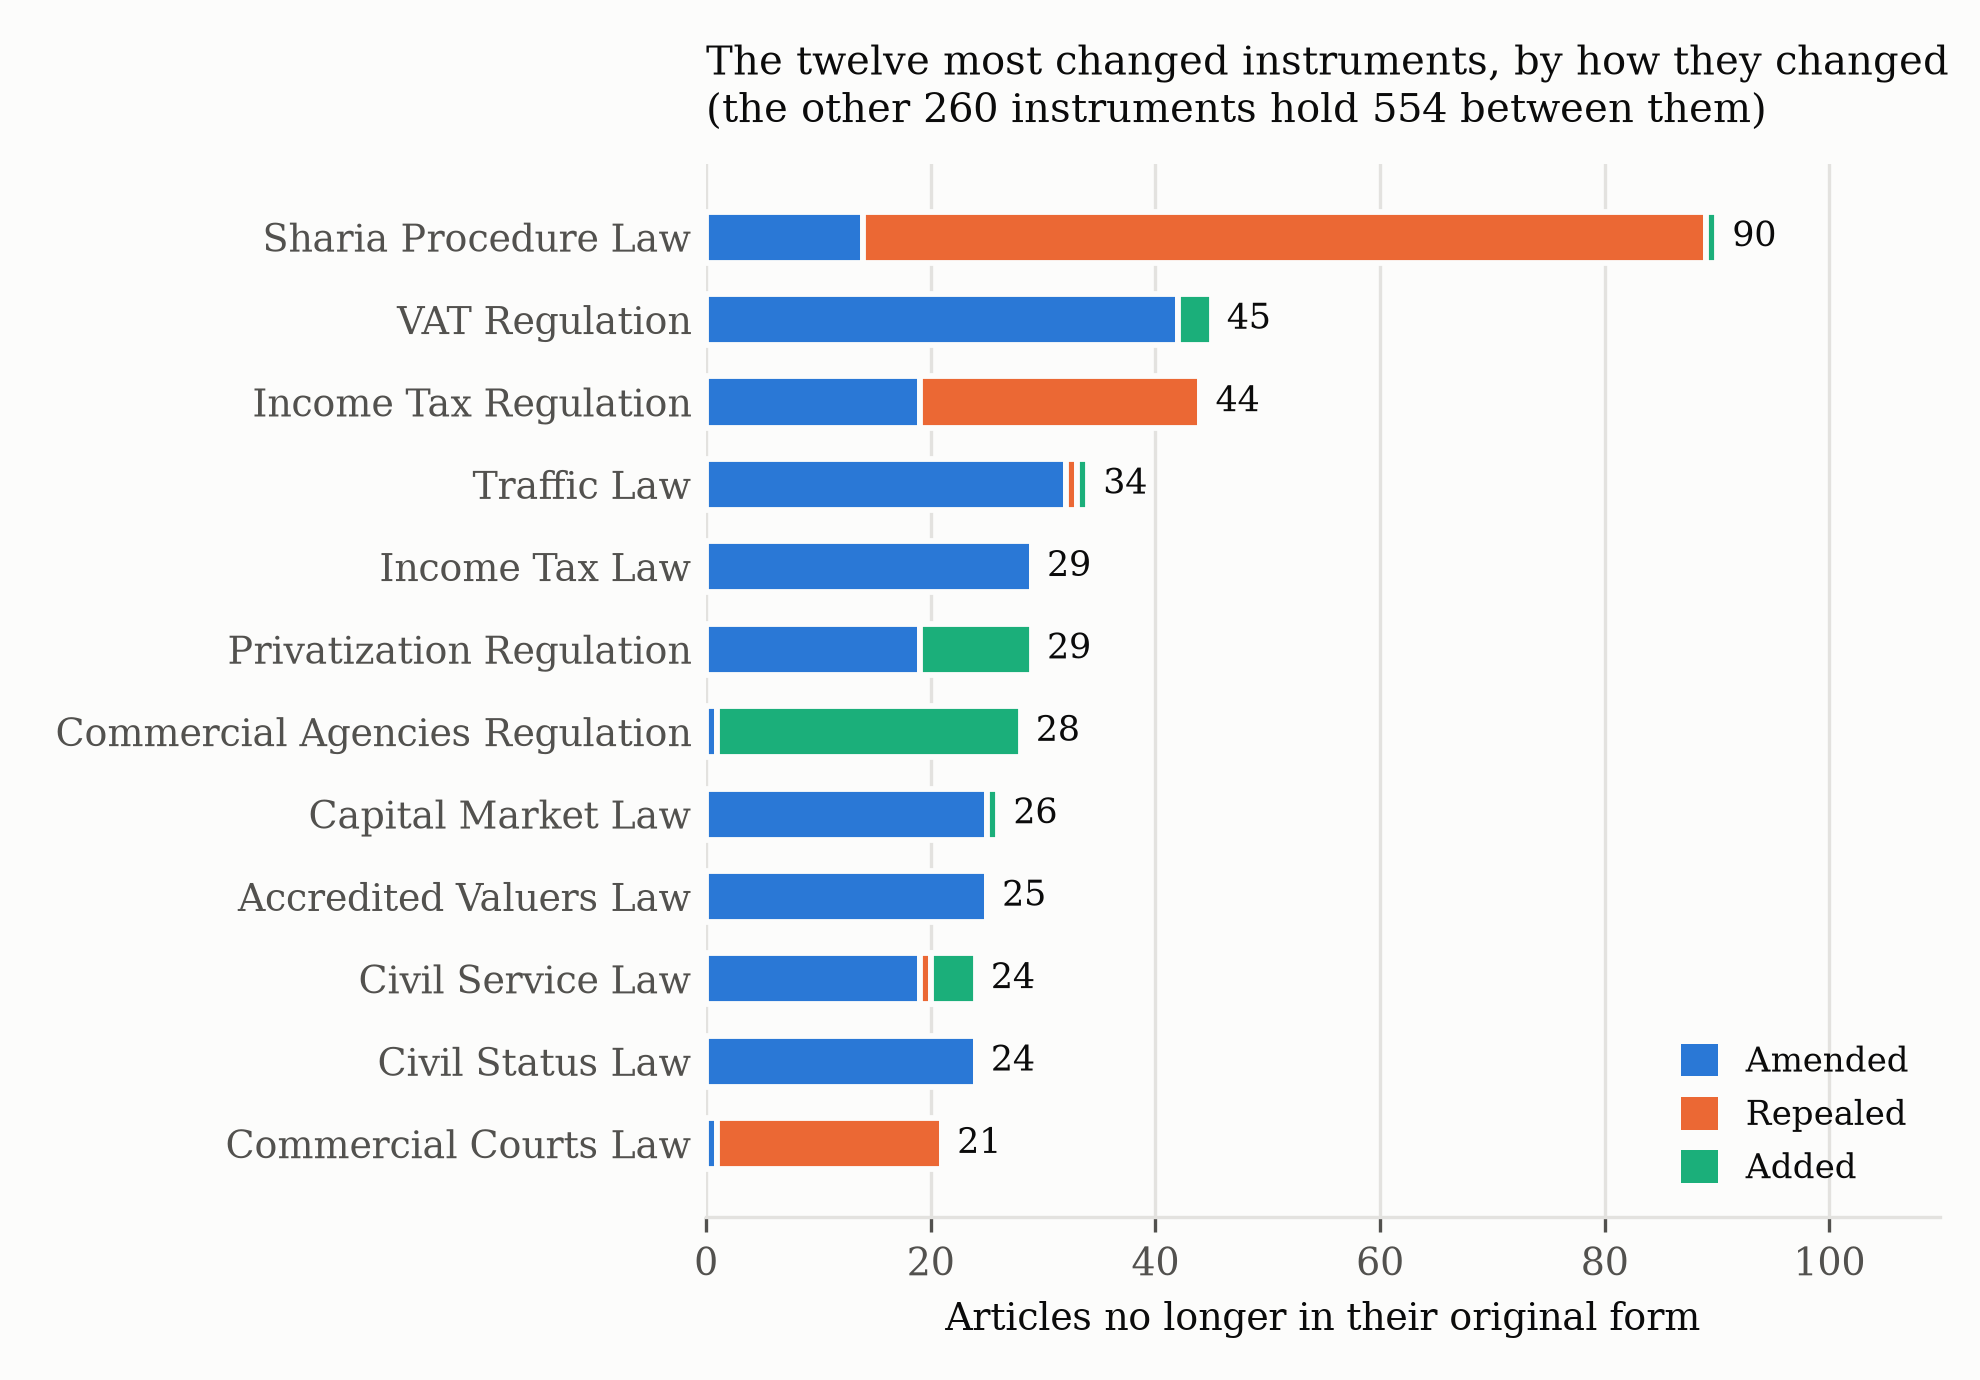
\includegraphics[width=\textwidth]{fig1_churn.png}
\caption{The twelve most changed instruments, split by how they changed. The
split is the point: the same total is reached by repeal in one instrument, by
addition in another, and by amendment in place in a third.}
\label{fig:churn}
\end{figure}

Table~\ref{tab:inventory} gives the aggregate. Three features deserve comment.

\textbf{The total is modest.} Of 13,089 articles, 12,109 stand as enacted.
That 7.4 per cent of a legal system's text has moved is neither alarming nor
negligible; it is the sort of figure that only becomes interesting when
disaggregated.

\textbf{The distribution is extreme.} A clear majority of instruments --- 160
of 272 --- record no change whatever, and the ten most changed instruments
hold better than a third of all changed articles. A Gini coefficient of 0.82
puts the concentration of legislative change on a par with the concentration
of citation reported for the same corpus, and the two concentrations turn out
to be related (section~\ref{sec:reliance}).

\textbf{Amendment is itself concentrated.} 179 distinct decrees and
resolutions account for the amendments that could be attributed, and the ten
most active account for 35.4 per cent of the article-amendment pairs. One
royal decree alone touches 81 articles. Legislative change in this system
arrives in occasional large consignments rather than as a steady drip --- a
shape that matters for anyone maintaining a downstream copy of the law, since
it means the maintenance burden is bursty rather than continuous.

\section{Instruments change in different ways}

Figure~\ref{fig:churn} separates the twelve most changed instruments into
amendment, repeal and addition, and the separation does real work. Three
signatures are visible, and they are three different legal events.

\paragraph{Hollowing out.} The Law of Sharia Procedure has 90 changed
articles, of which 75 are repeals --- 54 per cent of every repealed article in
the corpus, in one instrument. Fifty-eight of those repeals are the single
block of articles 101 to 158 removed by the decree that issued the Evidence
Law. The rest came from elsewhere, and the breakdown is a useful illustration
of the limits of the record: nine articles were repealed by a later decree,
one by an earlier one, and for seven the corpus records the repeal but no
repealing instrument at all.\footnote{Royal Decree M/43 (26/5/1443H) accounts
for 58 of the 75 --- articles 101--158; Royal Decree M/101 for 9 --- articles
227--235; Royal Decree M/93 for article 35. Seven further articles are
recorded as repealed with no decree attributed.} The
Commercial Courts Law shows the same signature at smaller scale: 20 of its 21
changed articles are repeals. This is
what it looks like when a subject matter is moved out of an instrument and
into a new one, leaving the original in force but emptied in the relevant part.
An instrument in this condition is the most dangerous kind for a reader,
because its size, its numbering and its continued force all suggest that it is
intact.

\paragraph{Accretion.} The Implementing Regulation of the Commercial Agencies
Law has 28 changed articles, of which 27 are additions and one an amendment.
Nothing was taken away; a regime was extended in place. The Implementing
Regulation of the Privatization Law shows a milder version, with 10 additions
against 19 amendments.

\paragraph{Tuning.} The VAT Regulation has 42 amendments, three additions and
no repeals; the Income Tax Law, 29 amendments and nothing else; the Civil
Status Law, 24 amendments and nothing else. Here the instrument's structure is
stable and its content is being adjusted --- the pattern one would expect of a
technical regime being kept current.

The fiscal instruments deserve a note of their own. Three of the twelve most
changed instruments are tax instruments --- the VAT Regulation, the Income Tax
Regulation and the Income Tax Law --- and between them they hold 118 changed
articles, an eighth of every changed article in the corpus. That is consistent with what one would expect of a system
that introduced value added tax in 2018 and has been adjusting the surrounding
regime since, and it is a reminder that a churn ranking is partly a map of
recent policy attention rather than of anything intrinsic to the instruments.

\section{What amendment does to the text}
\label{sec:magnitude}

For 87 amended articles the corpus records the wording that was replaced. That
is 11.9 per cent of all amended articles, and the sample is not random: it is
the articles whose official record happened to expose a prior version. Nothing
below should be read as an estimate for the other 88 per cent.

Within that sample, the median similarity between the current and the
superseded wording is 0.82, and the median change in length is four tokens.
Thirty-two of the 87 are near-identical (similarity at or above 0.90),
thirty-eight are moderate revisions, and seventeen are substantial rewrites
(below 0.50). Forty-eight articles grew and thirty-two shrank.

The distribution matters more than the median. Most amendment in this sample
is small --- a phrase substituted, a cross-reference updated, a threshold
changed. But roughly one amendment in five falls below 0.50, which for
articles of similar length means that about a third of the vocabulary has
gone.\footnote{Jaccard similarity is the intersection over the union, so for
two versions of equal length a score of 0.50 corresponds to roughly two-thirds
of tokens in common. A low score is a substantial revision; it is not a
synonym for `most of the article was replaced'.}

The extreme cases are extreme in substance and not only in wording. Article 72
of the Law of the Judiciary shrank from 29 tokens to 6 and shares three of
them with its predecessor. It formerly provided that the Deputy Minister of
Justice be chosen from among serving or former judges of a stated minimum
grade; it now provides only that the post is appointed at the excellent rank.
The qualification requirement was not reworded --- it was deleted, and the
similarity score is the trace of that deletion rather than its measure.

An amendment, in other words, is not a category with a typical magnitude. It
is a label covering interventions that range from a substituted preposition to
the removal of a substantive condition, and a system that tells a reader only
that an article `has been amended' has told them very little.

\section{Change and reliance}
\label{sec:reliance}

\begin{figure}[t]
\centering
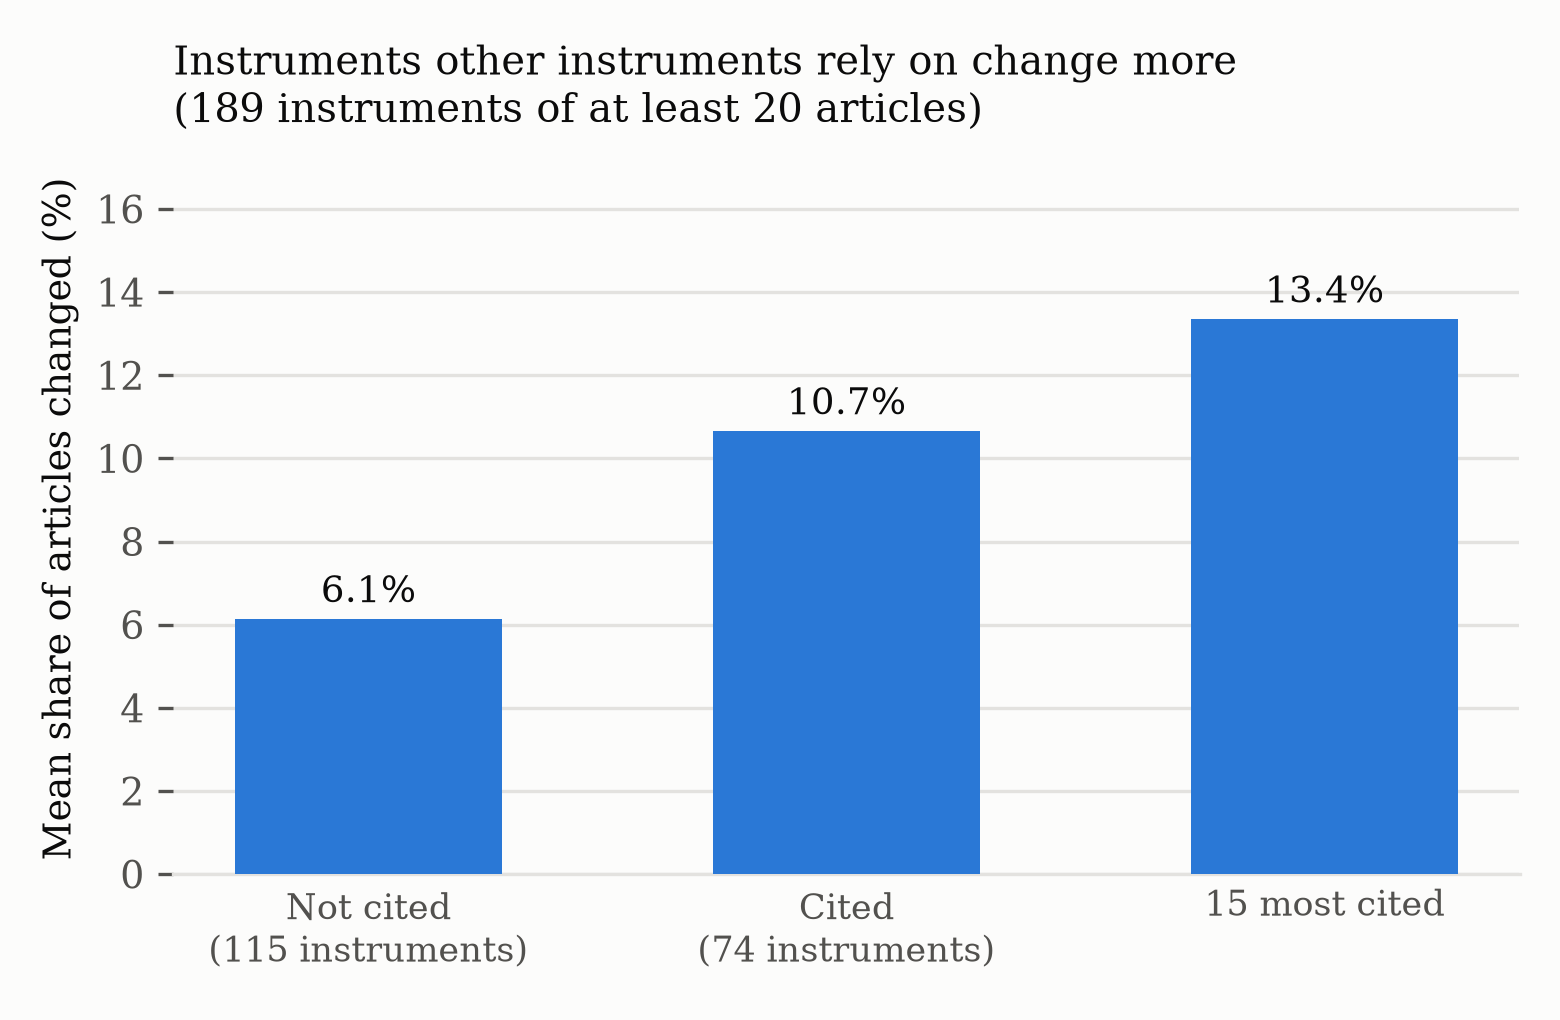
\includegraphics[width=0.78\textwidth]{fig2_citation_tiers.png}
\caption{Mean churn rate by citation tier, over the 189 instruments of at
least 20 articles. The three tiers are not disjoint: the fifteen most cited
are a subset of the cited.}
\label{fig:tiers}
\end{figure}

\subsection{Instruments others rely on change more}

Restricting to the 189 instruments with at least 20 articles --- below that a
churn rate is dominated by its denominator --- the instruments that other
instruments cite have a mean churn rate of 10.7 per cent, against 6.1 per cent
for the 115 instruments no other instrument cites. The fifteen most cited
average 13.4 per cent (Figure~\ref{fig:tiers}).

The gradient is clean, and it is also exactly the sort of result that deserves
scepticism. \textbf{Age is not controlled for.} An instrument enacted in
1426H has had two decades in which to be amended and two decades in which to
accumulate citations; an instrument enacted last year has had neither. The
gradient is therefore consistent with a real relationship between reliance and
change, with simple ageing, or with both. It cannot be separated here: the
corpus registry carries a publication date for two of its 291 tracks, so the
control is unavailable. Establishing which explanation holds would need a
dated corpus, and building one is a worthwhile piece of work in itself.

What can be said without the control is the descriptive fact, and it is not
trivial: the instruments a legal system's other instruments depend on are, as
things stand, the least stable part of it. Whatever the causal story, a reader
or a system that relies on the Companies Law or the Labour Law is relying on
text that moves more often than the average.

\subsection{Cross-instrument references are exposed; internal ones are not}

Of the corpus's cross-references, 2,624 resolve to a specific article whose
status is known. Of those, 233 --- 8.9 per cent --- point at an article that
has since been amended or repealed. Against a corpus base rate of 7.4 per cent
that is a ratio of 1.19: essentially nothing. Reported alone, `nine per cent
of citations point at changed law' would be a finding about the base rate
wearing a disguise.

The result appears when the references are split by type.

\begin{table}[t]
\centering
\small
\begin{tabular}{lrrr}
\toprule
\textbf{Reference type} & \textbf{Resolved} & \textbf{At changed text} &
\textbf{Share} \\
\midrule
To an article of another instrument & 86 & 15 & 17.4\% \\
To an article of the same instrument & 2,538 & 218 & 8.6\% \\
\midrule
Corpus base rate of changed articles & --- & --- & 7.4\% \\
\bottomrule
\end{tabular}
\caption{Exposure of cross-references to changed articles.}
\label{tab:exposure}
\end{table}

References an instrument makes to its own articles sit at the base rate: 8.6
per cent against 7.4. References it makes to another instrument's articles run
at 17.4 per cent --- twice the internal rate and 2.4 times the base rate.

The mechanism is not mysterious, and that is what makes the result useful. A
drafter amending an instrument has the whole of that instrument in front of
them. Internal cross-references are visible, and updating them is part of the
job. References \emph{into} the instrument from elsewhere are not visible ---
there is no index of them, and no step in the process at which anyone is asked
to look. The excess exposure is the measurable trace of a gap in the drafting
workflow rather than of anyone's carelessness.

Two cautions. The inter-instrument figure rests on 86 resolved references,
which is a small base; the corresponding confidence is correspondingly loose,
and the finding should be treated as an indication with a plausible mechanism
rather than a settled rate. And `points at an amended article' is not the same
as `is now wrong': an amendment may leave the cited proposition untouched.
What the number identifies is a set of references that nobody has checked, not
a set of errors.

\section{What follows}

\paragraph{Consolidation is not the whole answer.} The standard remedy for an
unreadable statute book is consolidation --- publishing the current text so
that a reader need not assemble it. Saudi practice already does this: the
official record shows the consolidated article. The Sharia Procedure Law shows
the limit of the remedy. Its consolidated text is accurate and it is
misleading, because an instrument that has lost a third of its articles to
repeal looks, consolidated, much like an instrument that has lost none. What a
reader needs is not only the current text but the fact of its distance from
the enacted one, and that is a presentational choice available today at no
legislative cost.

\paragraph{Reverse references are the missing tool.} If cross-instrument
references are the exposed ones, and they are exposed because a drafter cannot
see them, then the intervention is to make them visible. A reverse index ---
for any article, the list of provisions elsewhere that cite it --- is
computable from a corpus of the kind used here, and consulting it at the point
of amendment would convert an invisible risk into a checklist. This is the
same instrument the companion citation study proposed for a different purpose,
and it is worth noting that one artefact serves both.

\paragraph{`Amended' is too coarse a label to publish alone.} Section
\ref{sec:magnitude} found amendments ranging from a substituted phrase to the
replacement of ninety per cent of an article's wording, all carrying the same
label. Where the superseded text exists in the record, showing it --- or even
showing a similarity indicator --- costs nothing and tells a reader whether
the amendment they are looking at is worth reading.

\paragraph{For legal information systems.} Any system answering questions over
statutory text is answering from a snapshot. The results here say where the
snapshot decays fastest: not evenly, but in a small number of heavily-cited
instruments, and in bursts when a large amending decree lands. A refresh policy
that treats all instruments alike is doing too much work on the 58.8 per cent
that never change and too little on the handful that carry most of the
movement.

\section{Limitations}

\paragraph{The status layer is a transcription, not an audit.} Statuses come
from what the official record exposed for each article at the time the corpus
was built. Where the record is silent about an amendment, the article counts
as original here. The direction of that error is one-way: churn is understated,
not overstated.

\paragraph{Coverage is partial and uneven.} 272 of 291 tracks carry statuses,
and the 19 that do not are not a random sample. More importantly, the depth of
the amendment history varies by source: some instruments expose an event log,
some a prior version, most nothing at all. Every measure states the subset it
was computed on.

\paragraph{The magnitude sample is small and selected.} Eighty-seven articles,
11.9 per cent of amended articles, chosen by whether their source happened to
publish a prior version. It supports the claim that amendments vary enormously
in magnitude. It does not support any estimate of how the other 88 per cent are
distributed.

\paragraph{The reliance gradient is uncontrolled.} As section~\ref{sec:reliance}
states, age is a live alternative explanation and cannot be tested from this
corpus.

\paragraph{Dates are too sparse for a time series.} Only 175 of 759
article-amendment pairs carry a Gregorian date --- 23 per cent --- and the instruments that carry
dates are not representative. The apparent concentration of dated amendments in
a single year is an artefact of which sources expose dates, and no
year-on-year analysis is attempted here.

\paragraph{Reference resolution is automatic.} The cross-reference layer is
built by pattern extraction, and the companion citation study found that a
small share of resolved edges were misresolutions. Section~\ref{sec:reliance}'s
inter-instrument figure rests on 86 references, so a handful of bad
resolutions would move it.

\section{Conclusion}

Saudi legislation changes little in aggregate and very unevenly in
distribution. Of 13,089 articles, 973 are no longer in their original form; of
272 instruments, 160 have never changed at all, while ten hold a third of all
the change. Instruments do not merely change by different amounts, they change
in different ways --- hollowed out by repeal, extended by addition, or tuned in
place --- and the three are different legal events that a single count would
merge.

Two of the results bear on how a legal system is used rather than on how it is
written. The instruments other instruments rely on are the least stable, though
this article cannot separate that from ageing. And references from one
instrument into another are twice as exposed to changed text as an
instrument's references to itself --- an asymmetry with a mechanism a drafting
process could address, because it exists only because nobody can see the
references pointing at what they are about to amend.

The Law of Sharia Procedure remains the clearest case. It is in force, it is
cited, its numbering is intact, and seventy-five of its articles say nothing.
Nothing in how it is published conveys that. Now, at least, it can be counted.



\end{document}
